%% Basierend auf einer TeXnicCenter-Vorlage von Tino Weinkauf.
%%%%%%%%%%%%%%%%%%%%%%%%%%%%%%%%%%%%%%%%%%%%%%%%%%%%%%%%%%%%%%
\documentclass[a4paper,oneside,12pt]{report}
% Alternative Optionen:
%	Papiergröße: a4paper / a5paper / b5paper / letterpaper / legalpaper / executivepaper
% Duplex: oneside / twoside
% Grundlegende Fontgrößen: 10pt / 11pt / 12pt

\usepackage[ngerman]{babel}
\usepackage[utf8]{inputenc}
\usepackage[T1]{fontenc}

\usepackage{lmodern}

\usepackage{float}
\usepackage[export]{adjustbox}
\usepackage{graphicx} %%Zum Laden von Grafiken
\graphicspath{ {./images/} }
%\usepackage{subfig} %%Teilabbildungen in einer Abbildung
%\usepackage{pst-all} %%PSTricks - nicht verwendbar mit pdfLaTeX

%% Beachten Sie:
%% Die Einbindung einer Grafik erfolgt mit \includegraphics{Dateiname}
%% bzw. über den Dialog im Einfügen-Menü.
%% 
%% Im Modus "LaTeX => PDF" können Sie u.a. folgende Grafikformate verwenden:
%%   .jpg  .png  .pdf  .mps
%% 
%% In den Modi "LaTeX => DVI", "LaTeX => PS" und "LaTeX => PS => PDF"
%% können Sie u.a. folgende Grafikformate verwenden:
%%   .eps  .ps  .bmp  .pict  .pntg

%\usepackage{amsmath}
%\usepackage{amsthm}
%\usepackage{amsfonts}

%\usepackage{tabu}

%\usepackage{setspace}
%\singlespacing        %% 1-zeilig (Standard)
%\onehalfspacing       %% 1,5-zeilig
%\doublespacing        %% 2-zeilig

\usepackage{a4wide} %%Kleinere Seitenränder = mehr Text pro Zeile.
\usepackage{fancyhdr} %%Fancy Kopf- und Fußzeilen
%\usepackage{longtable} %%Für Tabellen, die eine Seite überschreiten

\usepackage{tabularx}
\usepackage{xltabular}

\usepackage{lscape}
\usepackage{pdflscape}

\usepackage{hyperref}
\usepackage{listings}
\usepackage{import}
\usepackage{pdfpages}

\usepackage{xcolor}
\usepackage{soul}

\usepackage{titling}

 %%Keine Kopf-/Fusszeilen auf den ersten Seiten.
\pagestyle{empty}

%% Deckblatt
%% ==> Schreiben Sie hier Ihren Text oder fügen Sie eine externe Datei ein.
\title{CKi ein CNN-Model in C++}
\author{Simeon Stix}
\date{\today}
\renewcommand{\maketitle}{
\begin{titlepage}
    \begin{center}
        \vspace*{1cm}
        
        \Huge
        \textbf{\thetitle}
        
        \vspace{0.5cm}
        \Large
        by \theauthor
        
        \vspace{1.5cm}
        
        \today
        
        \vfill
        
        Version: 1
        
        \vspace{1cm}
        
        Betreuer: Sven Nüesch
        
    \end{center}
\end{titlepage}
}

\begin{document}

\maketitle

%% Inhaltsverzeichnis 
\tableofcontents %Inhaltsverzeichnis
\cleardoublepage %Das erste Kapitel soll auf einer ungeraden Seite beginnen.

\pagestyle{plain} %%Ab hier die Kopf-/Fusszeilen: headings / fancy / ...

%% Hauptteil
%%Analyse
\chapter{Analyse}
\label{sec:Analyse}
\section{Aufgabenstellung}
\label{sec:AnalyseAufgabenstellung}
Die Aufgabe, die sich das Projekt CKi stellt, ist die Wissenserweiterung des Entwicklers. Dabei wird ein Programm geschrieben, welches einzelnen handgeschriebenen Ziffern erkennen kann. Dies geschieht mittels KI. Dabei wird die KI komplett vom Entwickler geschrieben. Da keine modernen externen Grundlagen verwendet werden, wird das Produkt, das Programm, nicht die Geschwindigkeit einer modernen KI erreichen. Dies spielt jedoch keine Rolle, da dieses Projekt nicht wegen des Endprodukts durchgeführt wird.

\section{Zielgruppe}
\label{sec:AnalyseZielgruppe}
Das Projekt CKi ist als solches nicht ausgelegt, einem realen Anwendungszweck zu entsprechen oder eine Lösung oder einen Lösungsansatz für einen solchen zu bieten. Diesbezüglich liegt der einzige Nutzen von CKi nicht in dessen Produkt, sondern nur im Wissensgewinn und Verständnis gewinn für den Entwickler in den Bereichen der künstlichen Intelligent oder genauer im Bereich des maschinellen Lernens mit einem \textit{Convolutional Neural Network}, der Realisation von Anwendungen mit C++ und dessen Möglichkeiten Hardware direkt in die programminternen Abläufe einzubinden. Somit richtet sich CKi nicht nach dem Grundsatz ein bestmögliches nutzbares Produkt zu sein, sondern lediglich nach dem grössten Wissensgewinn für den Entwickler. Nach diesem Grundsatz ist die resultierende Zielgruppe der Entwickler und vereint so multiple Rollen des Projektes CKi in einer Person.

\section{Anforderungen}
\label{sec:AnalyseAnforderungen}

\subsection{Must-haves}
\label{sec:AnalyseMustHaveS}
Die Must-haves wurden aus dem Themenblatt, welches am 15.09.2023 bei Walter Schnyder eingereicht wurde, übernommen und mit weiterführenden Elaborationen versehen.

\begin{itemize}
\item 
Rückgabe in Prozentwerten, die die Wahrscheinlichkeit der Übereinstimmung mit dem digitalen Gegenstück der handgeschriebenen Zahl abbildet. "Welche Zahl wurde (vermutlich) aufgeschrieben?"
\subparagraph{}
\textbf{Erläuterung:}
Da ein simples neuronales Netzwerk für maschinelles Lernen durch ein "Netz" aus Knotenpunkten gebaut wird und jeder dieser Knotenpunkte, auch die Knotenpunkte, welche bei einem solchen neuralen Netzwerk als Endschnittstellen fungieren, einzeln berechnet werden, erhält man, bei Anwendungsfall von CKi, eine multiple Anzahl von Prozentzahlen, welche zur Interpretation es gelieferten Endergebnisses verwendet werden können. Diese Rückgabe der einzelnen Prozentwerte erfolgt zum Beginn über eine Konsolenausgabe. Diese wird später, wie in \textit{"Nice-to-haves"} unter GUI erläutert, in ein grafisches Nutzerinterface integriert und zu diesem Zeitpunkt evtl. auch interpretiert (wobei die einzelnen Prozentwerte weiterhin einsichtig bleiben sollten).

\item CNN-Algorithmus (trainiert auf Zahlenwert)
\subparagraph{}
\textbf{Erläuterung:}
Ein CNN-Algorithmus oder auch Convolutional Neural Network wird beim maschinellen Lernen oft bei der Interpretation von Bildern genutzt. Dabei wird das Bild in kleinere Abschnitte unterteilt und „einzeln“ an den gehirnähnlich aufgebauten Algorithmus weitergegeben.
\begin{figure}[H]
\centering
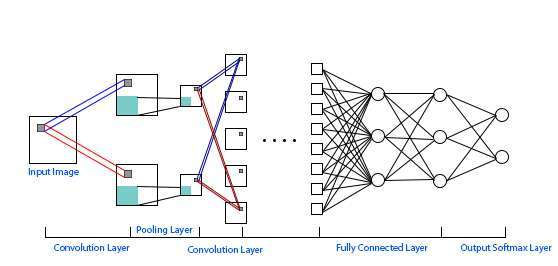
\includegraphics[scale=0.5]{CNN-model-with-several-convolution-and-pooling-layers-performed-alternately-combined.jpeg}
%von https://www.researchgate.net/publication/309751512/figure/fig1/AS:503017750437888@1496940185276/CNN-model-with-several-convolution-and-pooling-layers-performed-alternately-combined.png
\caption{CNN Model Aufbau Grafik}
\label{fig:AnalyseCNN-model-with-several-convolution-and-pooling-layers-performed-alternately-combined}
\end{figure}
Im Projekt CKi wird dieser wie im Themenblatt beschrieben mit Bild von einzelnen handgeschriebenen Ziffern trainiert.

\item Nutzer-Input → Nutzer darf eine Zahl zeichnen
\subparagraph{}
\textbf{Erläuterung:}
Ein solches CNN-Model zu erbauen und zu trainieren ist zwar die Grundlage für dieses Must-have, jedoch sollte das Produkt auch erprob bar sein. Diesbezüglich muss der Nutzer in der Lage sein, eine handschriftliche Ziffer an das neurale Netzwerk zu liefern. Hierbei ist die minimale Anforderung, dass der Nutzer in einer anderweitigen Applikation ein solches Bild erstellt hat und es nun interpretieren lassen kann. Wie in Nice-to-haves unter GUI beschreiben, wird diese Eingabemöglichkeit (eine Ziffer zu zeichnen oder eine schon vorhandene grafische Abbildung zu verwenden) in einem weiteren Entwicklungsschritt direkt in die grafische Nutzeroberfläche der Applikation integriert.

\end{itemize}

\subsection{Nice-to-haves}
\label{sec:AnalyseNiceToHaveS}
Die Nice-to-haves wurden aus dem Themenblatt, welches am 15.09.2023 bei Walter Schnyder eingereicht wurde, übernommen und mit weiterführenden Elaborationen versehen. Zudem behalte ich mir als Verfasser dieses Dokumentes, als Entwickler des Projektes CKi und als Zielgruppe des Projektes CKi vor, diese Liste in gegebene Falle zu erweitern.

\begin{itemize}
\item GUI
\subparagraph{}
\textbf{Erläuterung:}
Ein GUI (oder auch Graphical User-Interface) ist die grafische Nutzeroberfläche der Applikation. Da die Applikation primär dem Wissensgewinn gewidmet ist und dementsprechend nicht für den Nutzer optimiert wird, hat eine solche Erweiterung nur eine geringe Priorität. Diese Nutzeroberfläche wird selbst bei der Umsetzung in einer möglichst simplen Form gehalten. Dabei sollte es folgende Bestandteile beinhalten:
\begin{itemize}
\item Eine Möglichkeit für den Nutzer eine anderweitig gezeichnete Ziffer interpretieren zu lassen
\item Eine Möglichkeit für den Nutzer eine Ziffer zu zeichnen.
\item Eine weiter-interpretierte Ausgabe der Interpretation des CNN.
\item Eine Ausgabe des nicht interpretierten Prozentwertes der Interpretation des CNN.
\end{itemize}
Bis zu dem Punkt, wo ein GUI realisiert wurde und in den Einsatz gestellt wird, sind nicht alle dieser Funktionen über die Konsole (das Interface zum Programm, welches vor dem GUI zum Einsatz kommt) verfügbar.

\item GPU als Berechnungsplattform nutzen
\subparagraph{}
\textbf{Erläuterung:}
Die CPU in jedem Computer ist eine sehr „fokussierte“ Hardware, immer nur einen einzelnen Prozess kann diese berechnen. Dies ist für ein neuronales Netzwerk, welche Hunderte oder Tausende von Knotenpunkten in seinem Netzwerk hat und alle einzeln berechnet werden müssen, äusserst hinderlich. Die dezidierte Grafikkarte, wenn vorhanden, kann diesem Geschwindigkeitsverlust nachhelfen, da eine solche GPU in der Lage ist, tausende Berechnungen gleichzeitig zu tätigen.
Da im Projekt mit C++, einer Hardware-nahen Programmiersprache, gearbeitet wird, kann eine Anbindung an das Rechenpotential der GPU erreicht werden. Da dies jedoch ein äusserst schwieriger Prozess ist, sich diese Anbindung bei den unterschiedlichen Herstellern von GPUs unterscheiden kann und ich notwendig um ein funktionierendes CNN zu erstellen, wurde diese Optimierung als nicht notwendig eingestuft.
\end{itemize}

\subsection{Use Cases}
\label{sec:AnalyseUseCases}
Die hier aufgelisteten Use Cases entsprechen den Use Cases nach den Must-haves und sind diesbezüglich ohne die grafische Nutzeroberfläche. Dies kann dazu führen, dass ein endgültiges Produkt nicht mehr kohärent zu den Use Cases steht. Im Allgemeinen sollte aber selbst eine solche Inkohärenz nicht in extremer Weise auftreten, da die Bedienung der Applikation als Konsole als auch als grafische Oberfläche in ähnlicher Weise auftreten sollte.

\begin{landscape}
\begin{xltabular}{\linewidth}{|X|X|X|X|X|X|X|}
\hline
Nummer & Name & Akteur  & Ablauf & Nachbedingungen & Ausnahmen & Anmerkungen
\\\hline
1 & 
Interpretation & 
Nutzer, CNN  & 
Siehe Ablaufdiagramm "Interpretation" & 
Der Nutzer sollte in der Konsole eine Auflistung aller möglichen Ziffern (0-9) und deren entsprechenden Wahrscheinlichkeit sehen. Zudem kann der Nutzer auch die kongruierende Zahl zur höchsten Möglichkeit auf einer speziellen Zeile in der Konsole ablesen. & 
Bei der Interpretation von Nutzer-eigenen Abbildungen kann es zu multiplexen Fehlern kommen. Diese reichen von falschen Dateikodierung zu falscher Auflösung. Aufgrund dieser mannigfaltigen Möglichkeiten zu Fehlern können diese nicht alle hier erläutert werden. Eine Auflistung aller Fehler ist in der Dokumentation unter "\textit{Fehler}" zu finden. & 
Offiziell ist zwar Training keine Vorbedingung zu Testet, jedoch macht die Anwendung der Applikation keinen Sinn, wenn man nicht erwarten kann, dass man ein realistisches oder sinnvolles Ergebnis erhält.

\\\hline
2 &
Training & 
Nutzer, CNN  & 
Siehe Ablaufdiagramm "Training" & 
Der Nutzer erhält nach der Beendigung der Schulung des CNN-Models eine kurze Benachrichtigung, dass das Training abgeschlossen ist. Zudem erhält der Nutzer nach jedem einzelnen Datensatz den Output, dass nun x von y Datensätzen bearbeitet wurden.  & 
Hierbei kann es zu zwei Fehlern kommen. Dabei handelt es sich beides um Fehler bei der Datenbank. Der erste ist ein Fehler, wenn die benötigten "Tabellen" in der Datenbank nicht stimmig mit den Erwartungen sind und der andere, wenn keine Daten in der Datenbank zu finden sind. Für die genauen Fehlercodes ist die Dokumentation unter "\textit{Fehler}" zu kontaktieren. &
\\\hline
3 & 
Testen & 
Nutzer, CNN & 
Siehe Ablaufdiagramm "Testen" & 
Der Nutzer findet nach jedem Datensatz in der Test-Datenbank eine simple Gegenüberstellung der richtigen und der falschen interpretierten Ziffern. Diese weiterzuverarbeiten, ist dem Nutzer überlassen. Neben der Gegenüberstellung erhält der Nutzer auch die Benachrichtigung, dass nun x von y Datensätzen bearbeitet wurden. & 
Hier kann es zu zwei Fehlern kommen. Dabei handelt es sich beides um Fehler bei der Datenbank. Der erste ist ein Fehler, wenn die benötigten "Tabellen" in der Datenbank nicht stimmig mit den Erwartungen sind und der andere, wenn keine Daten in der Datenbank zu finden sind. Für die genauen Fehlercodes ist die Dokumentation unter "\textit{Fehler}" zu kontaktieren. & 
Bei den Testdaten würde es evtl. Sinn machen, die einzelnen Konsolen Outputs auch in einer CSV-Datei festzuhalten, wobei dies mit Pipes in der Konsole dem Nutzer bereits offensteht.  
Offiziell ist zwar Training keine Vorbedingung zu Testet, jedoch macht das Testen nur begrenze Sinn, wenn es noch nichts gibt, was sich zu testen lohnt. 
\\\hline
\end{xltabular}
\label{tab:AnalyseUseCases}
\end{landscape}

\subsection{Use Case Diagramme}
\label{sec:AnalyseUseCaseDiagramme}
\begin{figure}[H]
\centering
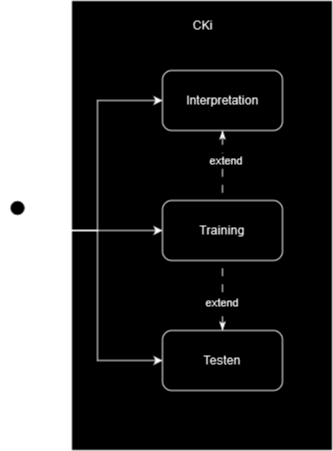
\includegraphics[height=0.5\paperheight]{usecase.png}
\caption{Use-Case-Diagramm}
\label{fig:analyseusecase}
\end{figure}

\subsection{Ablaufdiagramme}
\label{sec:AnalyseAblaufdiagramme}

\subsubsection{Interpretation}
\label{sec:AnalyseInterpretation}
\begin{figure}[H]
\centering
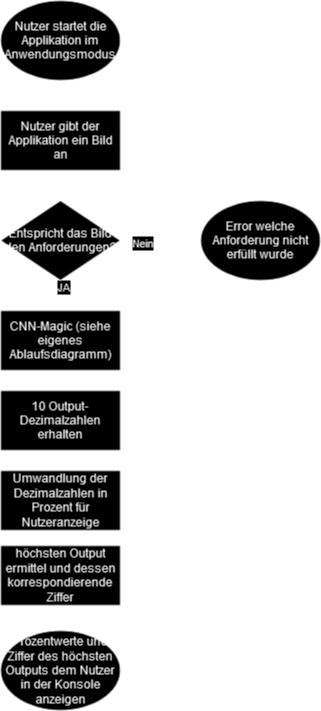
\includegraphics[height=0.5\paperheight]{ablauf-interpretation.png}
\caption{Ablaufdiagramm für die Interpretation von Nutzer-gelieferten Einzelbildern}
\label{fig:analyseablauf-interpretation}
\end{figure}


\subsubsection{Training}
\label{sec:AnalyseTraining}
\begin{figure}[H]
\centering
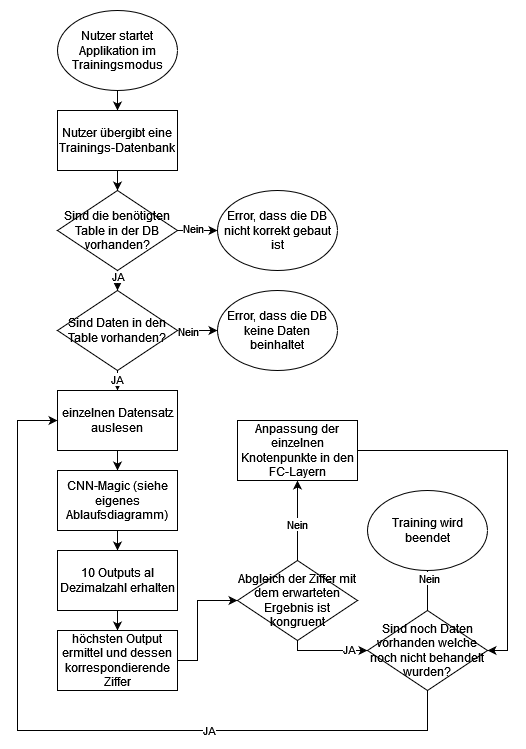
\includegraphics[height=0.5\paperheight]{ablauf-training.png}
\caption{Ablaufdiagramm vom Training des CNN}
\label{fig:analyseablauf-training}
\end{figure}


\subsubsection{Testen}
\label{sec:AnalyseTesten}
\begin{figure}[H]
\centering
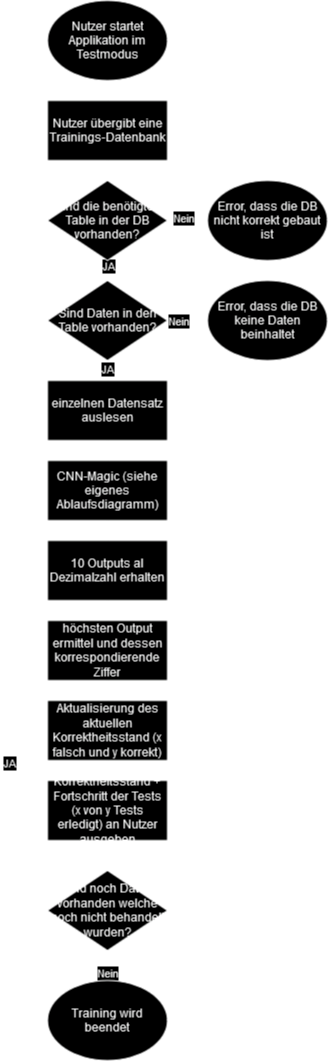
\includegraphics[height=0.5\paperheight]{ablauf-testen.png}
\caption{Ablaufdiagramm von einem Test des CNN}
\label{fig:analyseablauf-testen}
\end{figure}


\subsubsection{CNN-Magic}
\label{sec:AnalyseCNN-Magic}
\begin{figure}[H]
\centering
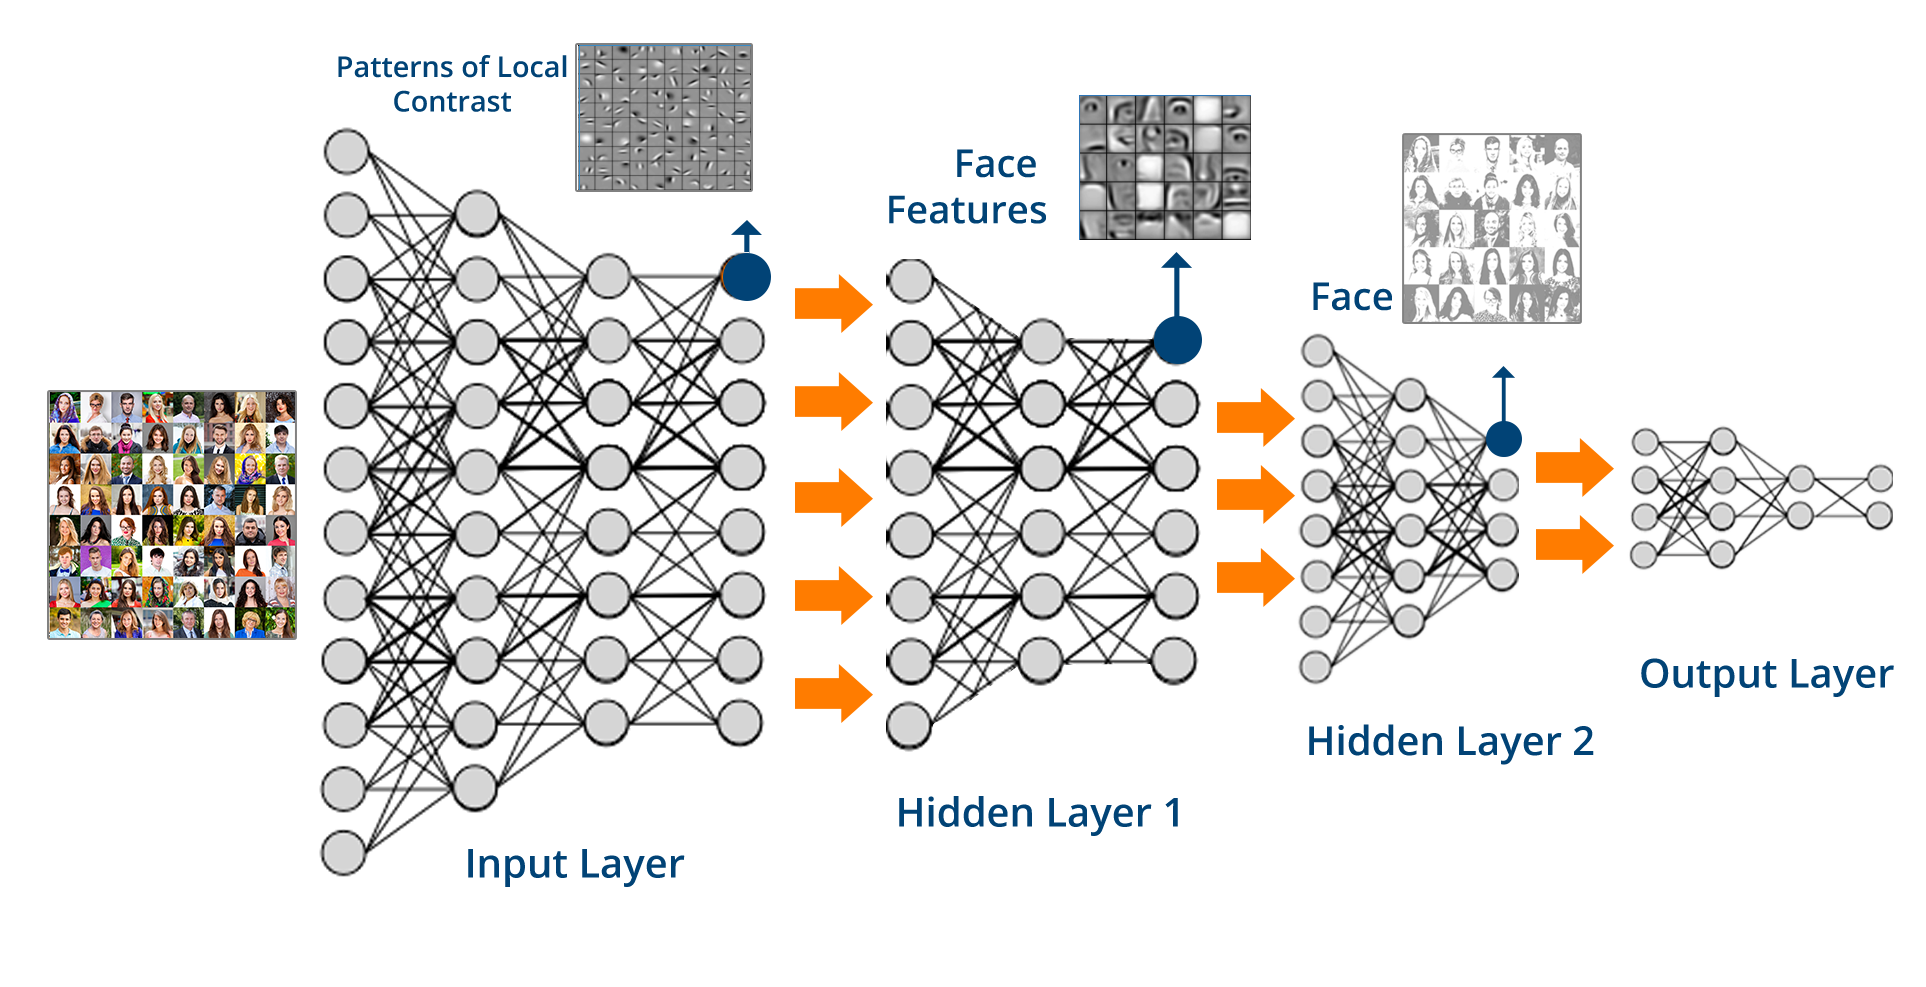
\includegraphics[width=\linewidth]{1 RXJ6tAmfN1AYLQr7p48L7w-631173908.png}
% von https://external-content.duckduckgo.com/iu/?u=https%3A%2F%2Fmiro.medium.com%2Fproxy%2F1*RXJ6tAmfN1AYLQr7p48L7w.png&f=1&nofb=1&ipt=4eb63d23b17398cd376f86942611c6a9fda3b4520fc8eb09e736d7f19f0d276d&ipo=images
\caption{Visuelle Darstellung der Funktionsweise eines CNN}
\label{fig:analyse1RXJ6tAmfN1AYLQr7p48L7w-631173908}
\end{figure}

\section{Umsetzung}
\label{sec:AnalyseUmsetzung}
Wie im Themenblatt vom 15.09.2023 wird für die Umsetzung reines C++ verwendet.

\subsection{Entwicklungsumgebung}
\label{sec:AnalyseEntwicklungsumgebung}
Bei der Entwicklungsumgebung wird das JetBrains Produkt \textbf{CLion} zum Einsatz kommen. Dieses beinhaltet alle benötigten Funktionalitäten, die bei der Entwicklung des Produktes nötig sind. Gegebenen Falles könnte noch \textbf{SQLite Browser} zur Verwendung kommen, da dieses ein besseres (und für den Entwickler ein gewohntes) Interface zur Handhabung von lokalen Datenbanken bietet. Für die Version Control des Projektes wird lokal \textbf{Git} verwendet und zur Sicherung in der Cloud wird sowohl \textbf{GitHub} als auch \textbf{GitLab} verwendet. Die Entwicklungsumgebung mit IDE und Version Control wird primär auf dem Betriebssystem Windows verwendet. Es kann jedoch nicht garantiert sein, dass die Entwicklung nicht teilweise unter einer Distribution von Linux ablaufen wird. Hierbei sollten (evtl. abgesehen von der GUI) keine Kompatibilitätsprobleme mit sich führen. 
\subsubsection{Auflistung Versionen}
\label{sec:AnalyseDevEnvAuflistung}
\begin{itemize}
\item JetBrains Toolbox 2.1.1.18388, Windows 11, x64
\item CLion (von JetBrains Toolbox) 2023.2.2
\item Git 2.39.2.windows.1
\end{itemize}

\subsection{CNN}
\label{sec:AnalyseCNN}
\subsubsection{Grundlagen}
\label{sec:AnalyseGrundlagen}
Der Kern des CNN lässt sich in drei unterschiedliche Arten von Schichten aufteilen. Zusätzlich gibt es noch zwei zusätzliche "Hilfs-"Schichten, welche für die Ein- und Ausgaben zuständig sind. 
Die \textit{Eingabeschicht} ist eine dieser zwei erwähnten Schichten. Diese akzeptiert im Falle von CKi jeweils ein Bild von speziell definierten Grössen und nimmt, gibt jeder Pixel in Graustufen (Dies ist entscheidend, weil so der Farbwert des Pixels von drei, zwei Byte grossen Zahlen zu nur einer zwei Byte grossen Zahl reduziert wird.) als ein sogenanntes Eingabeneuron. 
Auf die Eingabeschicht folgt die \textit{Convolutional Layers} oder auch \textit{Faltungsschichten}. Diese Faltungsschichten sind einer der Schlüsselbestandteile eines CNN. Die Convolutional Layer dienen dazu, bestimmte Merkmale und Schlüsselelemente aus dem Bild zu extrahieren. Hierbei wird bei jedem der Convolutional Layer eine 
mathematische Faltungsoperationen durchführt. 
Nach den Faltungsschichten kommen die simplen \textit{Pooling-Schichten}. Bei einer Pooling-Schicht wird die Dimension eines Bildes reduziert (Downsampling). Dies kann durch zwei Arten geschehen, entweder durch Max-Pooling, dabei wird aus einer Liste von Werten nur der höchste übermittelt oder durch Durchschnitts-Pooling, wobei der Durchschnitt dieser Liste berechnet und übermittelt wird. Durch diese Datenreduktion wird Rechenleistung gespart und so das Ergebnis schneller und stabiler geliefert. 
Vor der Ausgabeschicht gibt es noch die \textit{FC Layers} oder auch \textit{Vollständig verknüpfte Schichten}. Bei diesen ist jeder Knotenpunkt mit jedem Knotenpunkt in der nächsten Schicht verbunden. Dies ist das Herz des gesamten Models. Dabei wird in jedem Knotenpunkt ein neuer Wert berechnet, um in der letzten Schicht, der \textit{Ausgabeschicht} diese in Wahrscheinlichkeit zu "konvertieren".

\subsubsection{Implementation}
\label{sec:AnalyseImplementation}
Bei der Implementation eines CNN-Models wurde für CKi der Entschluss getroffen, eine C++-Klasse für jede benötigte Art von Layer zu schreiben. Danach muss ein Grundgerüst, eine Main-Klasse realisiert werden, die alle Klassen miteinander kombiniert. Dies erleichtert es in einem späteren Schritt die grosse Umstellung von einer Konsolen-Anwendung hin zu einer grafisch passierten Anwendung (auch wenn immer noch grosse Teile der Main-Klasse ausgetauscht werden müssen.). Für die Speicherung der Berechnungswerte für die FC-Layer ist die Abwägung zu treffen, ob es sinnvoll ist, diese in einer lokalen Datenbank zu speichern oder in eine konkret hierfür entworfene Datei zu schreiben.

\subsection{Testdaten}
\label{sec:AnalyseTestdaten}
Die Testdaten für CKi können in unzähliger Ausführung auf \href{https://www.kaggle.com/}{Kaggle} gefunden werden.

\subsubsection{Speicherung}
\label{sec:AnalyseSpeicherung}
Im gegebenen Fall würde es für die Schulung, des CNN, Sinn ergeben, die einzelnen Bilder nicht über Ordner- oder Archivstrukturen zu speichern, sondern in eine oder mehrere lokale Datenbanken abzuspeichern.

\section{Abwägung des Nutzens und der Alternativen}
\label{sec:AnalyseNutzwertanalyseDerLösungsvarianten}
\subsection{Alternativen}
\label{sec:AnalyseAlternativen}
Die möglichen Alternativen zu einer kompletten Realisation eine CNN oder irgendeinem neuronalen Netzwerk in C++ ohne Bibliotheken oder Frameworks für neuronale Netze sind endlos. 
Selbst wenn man bereits bestehende Produkte begutachtet, wird man auf GitHub schnell fündig. Bei einer Suche auf GitHub mit dem Query "mnist digit recogniser" findet man nach Stand 20.10.2023 02:13 178 Repositorien (je eines in C, C++, C\#, Rust, drei in Java + Kotlin und 53 in Python).
Selbst wenn man unter dem Beschluss steht, dass man das CNN selber bauen wolle, würde man für jede beliebige Sprache eine Bibliothek oder Framework finden, die einem diese Aufgabe erleichtern würde.

\subsection{Kosten}
\label{sec:AnalyseKosten}
Bezüglich der Kosten kann das Projekt CKi nicht mit den Alternativen mithalten. C++ ist keine Sprache, in welcher man schnell ein Produkt hervorbringt. Dies belegen etliche Studien und Artikel (
\href{https://www.cs.bsu.edu/homepages/dmz/cs697/langtbl.htm}{Programming Languages Table}, 
\href{https://citeseerx.ist.psu.edu/viewdoc/download?doi=10.1.1.113.1831&rep=rep1&type=pdf}{An Empirical Comparison of Seven Programming Languages},
\href{https://haslab.github.io/SAFER/scp21.pdf}{Programming Languages by Energy Efficiency}, 
\href{https://stackoverflow.com/questions/1894453/development-time-in-various-languages}{Development time in various languages})
Zudem, dass keine dezidierten Bibliotheken für maschinelles Lernen zum Einsatz kommen, erhöht den Entwicklungsaufwand, Zeitaufwand und so die Kosten.
Wenn man die Stundenzahl aus der Planung mit einem Stundensatz von 50 CHF quantifizieren, käme man auf einen gesamten Kostenaufwand von 8'600.-. Zuzüglich kämen noch Hardware Anschaffungen für die Entwicklung, diese können jedoch im Falle vom Projekt CKi vernachlässigt werden.  

\subsection{Nutzen}
\label{sec:AnalyseNutzen}
Wie bereits im Abschnitt \ref{sec:Zielgruppe} erwähnt, ist dieses Produkt auf den Wissensgewinn ausgerichtet und nicht auf das Produkt selbst. Dementsprechend ist in der geplanten Umsetzung der Projektes CKi der maximale Nutzen gewährleistet. Leider lässt sich dieser Nutzen nicht/schlecht quantifizieren.

\subsection{Effektivität}
\label{sec:AnalyseEffektivität}
Der Vergleich in Effektivität der Anwendung, die aus dem Projekt CKi resultiert und den professionell entwickelten Bibliotheken in Python, etc. zieht, wird CKi selbst mit GPU-Berechnung und dem Geschwindigkeitsvorteil von C++ gegen diese Bibliotheken in Bezug auf Run-Time-Length verlieren.

\subsection{Vergleich}
\label{sec:AnalyseVergleich}

\begin{xltabular}{\linewidth}{|X|X||X|X|}
\hline
\multicolumn{2}{|c||}{Bestehendes Produkt} & \multicolumn{2}{c|}{Eigene Kreation}
\\\hline
Sektion & Anzahl & Sektion & Anzahl
\\\hline
Anschaffungskosten & 0.- Fr.  & Kreation & 8'600.- Fr.
\\\hline
Wiederholende Kosten & 0.- Fr. & wiederholende Kosten & 0.- Fr.
\\\hline\hline
Absolut & 0.- Fr. & absolut & 8'600.- Fr.
\\\hline
\end{xltabular}
\label{tab:AnalyseVergleichTable}

Eine kurze Zusammenfassung der Kosten-Nutzen-Analyse zeigt den desolaten Zustand von CKi.\
Es werden Kosten für die Arbeitszeit von 8'600 CHF anfallen. Die Effektivität ist niedriger, als wenn dasselbe Produkt mit einer vorhandenen Bibliothek geschrieben werden würde (und die Entwicklungsdauer wäre ebenfalls geringer). Der Nutzen des Endproduktes ist nichtig, da dieses nie zur wirklichen Anwendung kommen wird. Weiters gibt es unzählige kostenlose Alternativen, die es nur zu verwenden gilt.\
Das Projekt CKi kann und wird sich nur auf den Wissensgewinn für den Entwickler stützen, in der Hoffnung, dass dieser die Kosten-Politik aufwiegen wird.

\subsection{Nutzwertanalyse}
\label{sec:AnalyseNutzwerkanalyse}
Bei der Nutzwertanalyse werden unterschiedliche Alternativen systematisch und statistisch nach gewissen Kategorien verglichen. Konkret werden hier unterschiedliche Möglichkeiten der Implementierung miteinander verglichen, dabei wird eine Punkteskala von eins bis zehn verwendet. Wichtig bei der Implementation ist es, dass eine höhere Punktzahl nicht bedeutet, wie hoch diese Kategorie ist. Eine Entwicklungsdauer von 10 bedeutet nicht, dass diese besonders lang ist, sondern dass diese Option im Bereich Entwicklungsdauer zehn Punkte erhalten hat (also besonders schnell zum Implementieren ist).

\begin{xltabular}{\linewidth}{|l|l||c|c||c|c|}
\hline
\multicolumn{2}{|X||}{Kriterien} & \multicolumn{2}{X||}{Python mit Tensflow} & \multicolumn{2}{X|}{C++}
\\\hline
Entwicklungsdauer & 10 \% & 10 & 1 & 2 & 0.2
\\\hline
Komplexität & 15 \% & 10 & 1.5 & 4 & 0.6
\\\hline
Sprachkenntnisse & 10 \% & 3 & 0.3 & 4 & 0.4
\\\hline
Frust & 10 \% & 5 & 0.5 & 7 & 0.7
\\\hline
Typisierung & 5 \% & 1 & 0.05 & 9 & 0.45
\\\hline
Run-Time-Length & 10 \% & 10 & 1 & 9 & 0.9
\\\hline
Testing & 5 \% & 6 & 0.3 & 7 & 0.35
\\\hline
Objektorintiert & 5 \% & 5 & 0.25 & 9 & 0.45
\\\hline
Wissensgewinn & 30 \% & 2 & 0.6 & 10 & 3
\\\hline\hline
Total & 100 \% & 52 & 5.5 & \hl{61} & \hl{7.05}
\\\hline
\end{xltabular}
\label{tab:AnalyseNutzwertanalyse}




%%Planung
\chapter{Planung}
\label{sec:Planung}
\section{Rollenverteilung}
\label{sec:PlanungRollenverteilung}

	\begin{xltabular}{\linewidth}{|l|X|}
		\hline
		\textbf{Rolle} & \textbf{Person}
		\\\hline
		Leiter & Simeon Stix
		\\\hline
		Entwickler & Simeon Stix
		\\\hline
		Betreuer & Sven Nüesch
		\\\hline
	\end{xltabular}
	\label{tab:planungrollenverteilungtable}
	\addcontentsline{lot}{table}{\protect\numberline{\thetable} Rollenverteilung im Projekt CKI}
\section{Aufgabenliste} 
\label{sec:PlanungAufgabenliste} 
\begin{enumerate} 
	\item \textbf{\emph{Planung:}} 
	\begin{itemize} 
		\item Aufgabenliste erstellen
		\item Zeiteinteilung 
		\item Meilensteine definieren 
		\item Gantt erstellen 
	\end{itemize} 
	\item \textbf{\emph{Analyse:}} 
	\begin{itemize} 
		\item Recherche CNN 
		\item Recherche Testdaten 
		\item Recherche C++ Details 
		\item Anforderungen definieren 
		\item Use Cases 
		\item weitere Analysen 
		\item Analyse schreiben
	\end{itemize} 
	\item \textbf{\emph{Design:}} 
	\begin{itemize} 
		\item GUI konzipieren 
		\item Wireframes zeichnen 
		\item Konsolenbefehle definieren 
		\item Konsolen-Output definieren 
	\end{itemize}
	\item \textbf{\emph{Realisation:}} 
	\begin{itemize} 
		\item Input Layer realisieren 
		\item Convolutional Layer realisieren 
		\item Pooling Layer realisieren 
		\item Dense Layer Klasse schreiben 
		\item Output Layer erstellen 
		\item CNN-Model erstellen 
		\item CNN-Model trainieren 
		\item GUI auf CNN-Model setzen 
		\item GPU-Anbindung implementieren 
		\item Kommentare schreiben 
		\item weitere Verbesserungen vornehmen 
		\item Puffer-Zeit fürs Programmieren 
	\end{itemize} 
	\item \textbf{\emph{Dokumentieren:}} 
	\begin{itemize} 
		\item Schreiben 
	\end{itemize} 
	\item \textbf{\emph{Testen:}} 
	\begin{itemize} 
		\item Testliste kreieren 
		\item Tests implementieren 
		\item Tests durchführen 
	\end{itemize} 
	\item \textbf{\emph{Deployment:}} 
	\begin{itemize} 
		\item Projekt als EXE bauen 
		\item Build-Anleitung kreieren 
	\end{itemize} 
	\item \textbf{\emph{Präsentation:}} 
	\begin{itemize} 
		\item Präsentation erstellen 
	\end{itemize}
\end{enumerate} 
\section{Meilensteine} 
\label{sec:PlanungMeilensteine} 

\begin{xltabular}{\linewidth}{|X|X|} 
	\hline Meilenstein-Name & Datum 
	\\\hline Vorbereitungen abgeschlossen & 20.10.2023 
	\\\hline CNN-Model Kreation abgeschlossen & 10.11.2023 
	\\\hline Dokumentation abgeschlossen & 01.12.2023 
	\\\hline Produkt abgeschlossen & 05.01.2024 
	\\\hline Projekt abgeschlossen & 10.02.2024 
	\\\hline \hl{Projekt abgegeben} & \hl{23.02.2024} 
	\\\hline 
\end{xltabular}
\addcontentsline{lot}{table}{\protect\numberline{\thetable}Meilensteine}

\label{tab:PlanungMeilensteineTable}
\section{Gantt} 
\label{sec:PlanungGantt} 
\begin{landscape}
	\addcontentsline{lof}{figure}{\protect\numberline{\thefigure}Das Gantt-Diagramm für das Projekt CKI}
	\begin{figure}[htbp]
		\centering
		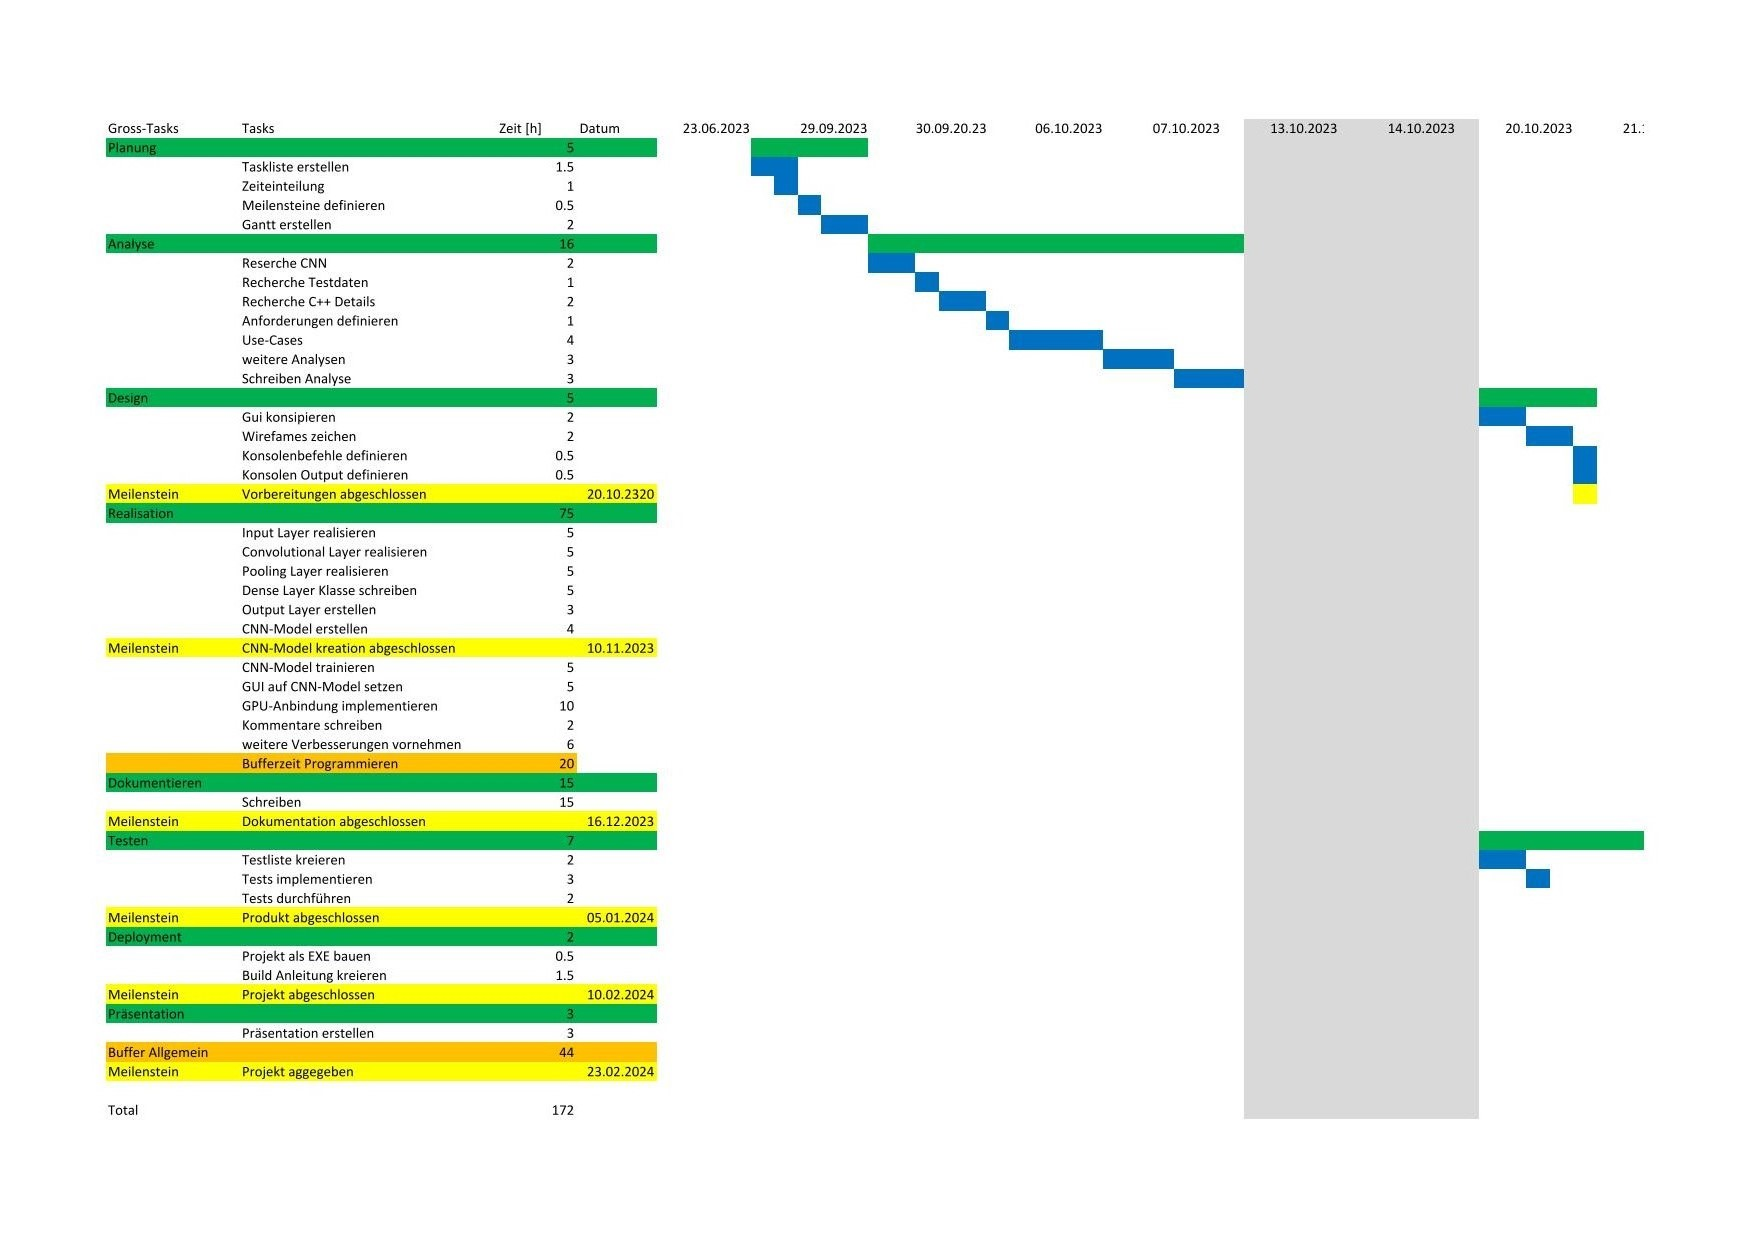
\includegraphics[width=\linewidth, height=\textheight, keepaspectratio]{gantt1_turned.jpg}
		\label{fig:gantt1}
	\end{figure}

	\begin{figure}[htbp]
		\centering
		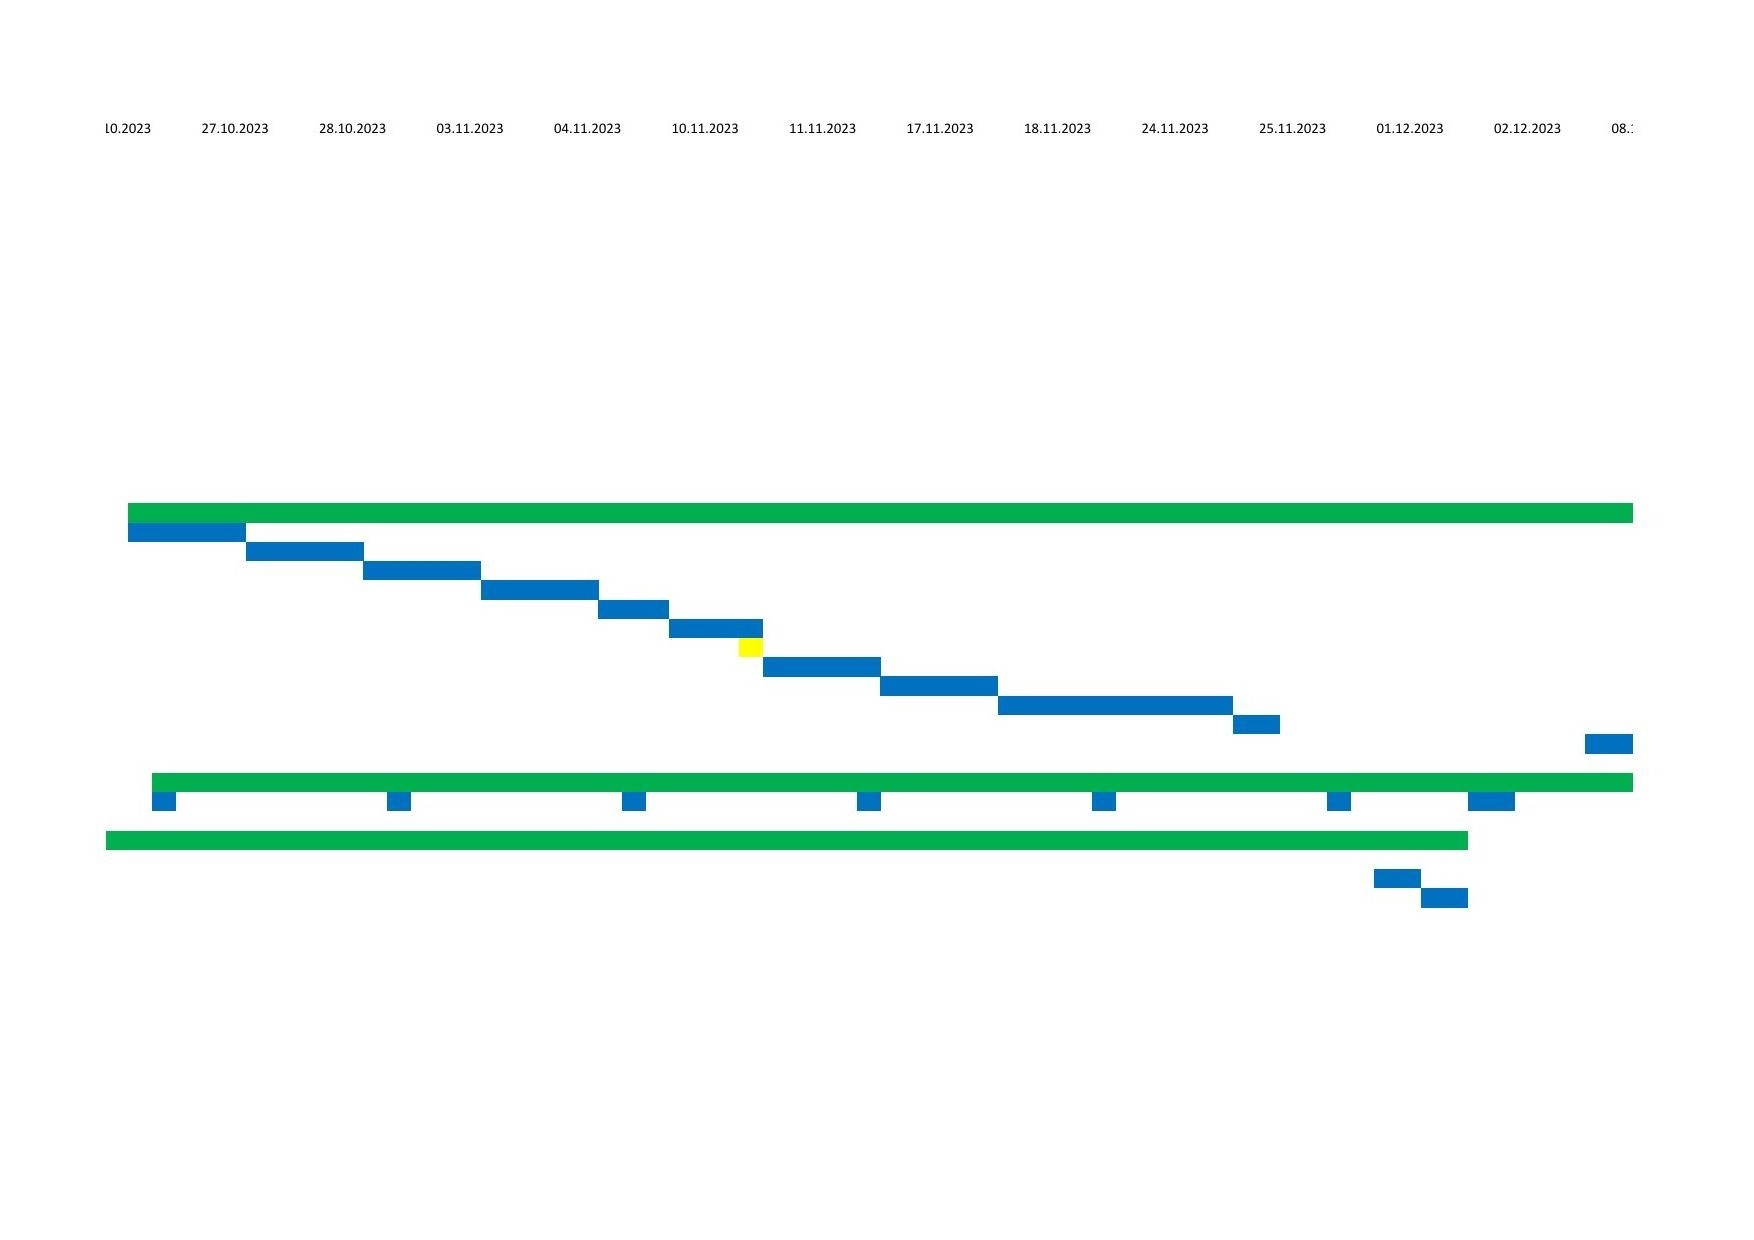
\includegraphics[width=\linewidth, height=\textheight, keepaspectratio]{gantt2_turned.jpg}
		\label{fig:gantt2}
	\end{figure}

	\begin{figure}[htbp]
		\centering
		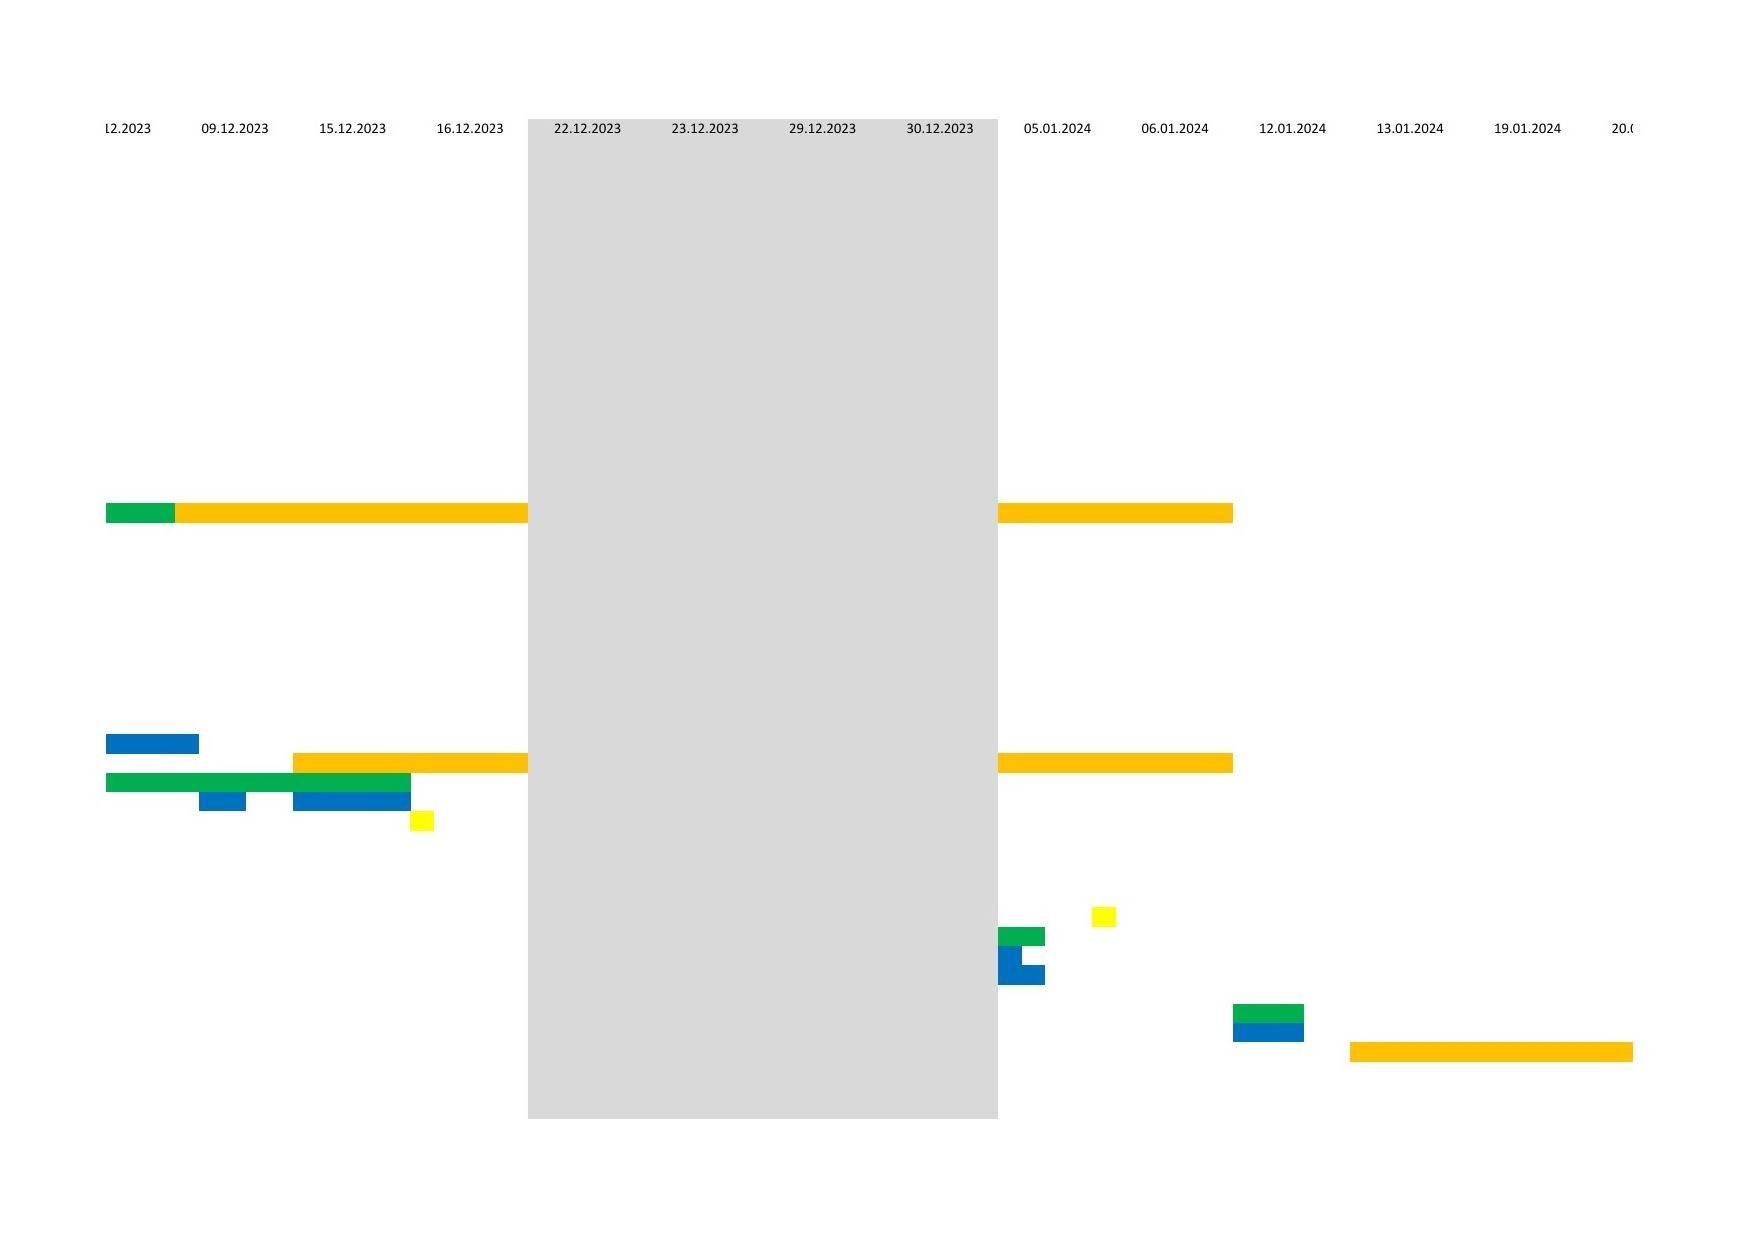
\includegraphics[width=\linewidth, height=\textheight, keepaspectratio]{gantt3_turned.jpg}
		\label{fig:gantt3}
	\end{figure}

	\begin{figure}[htbp]
		\centering
		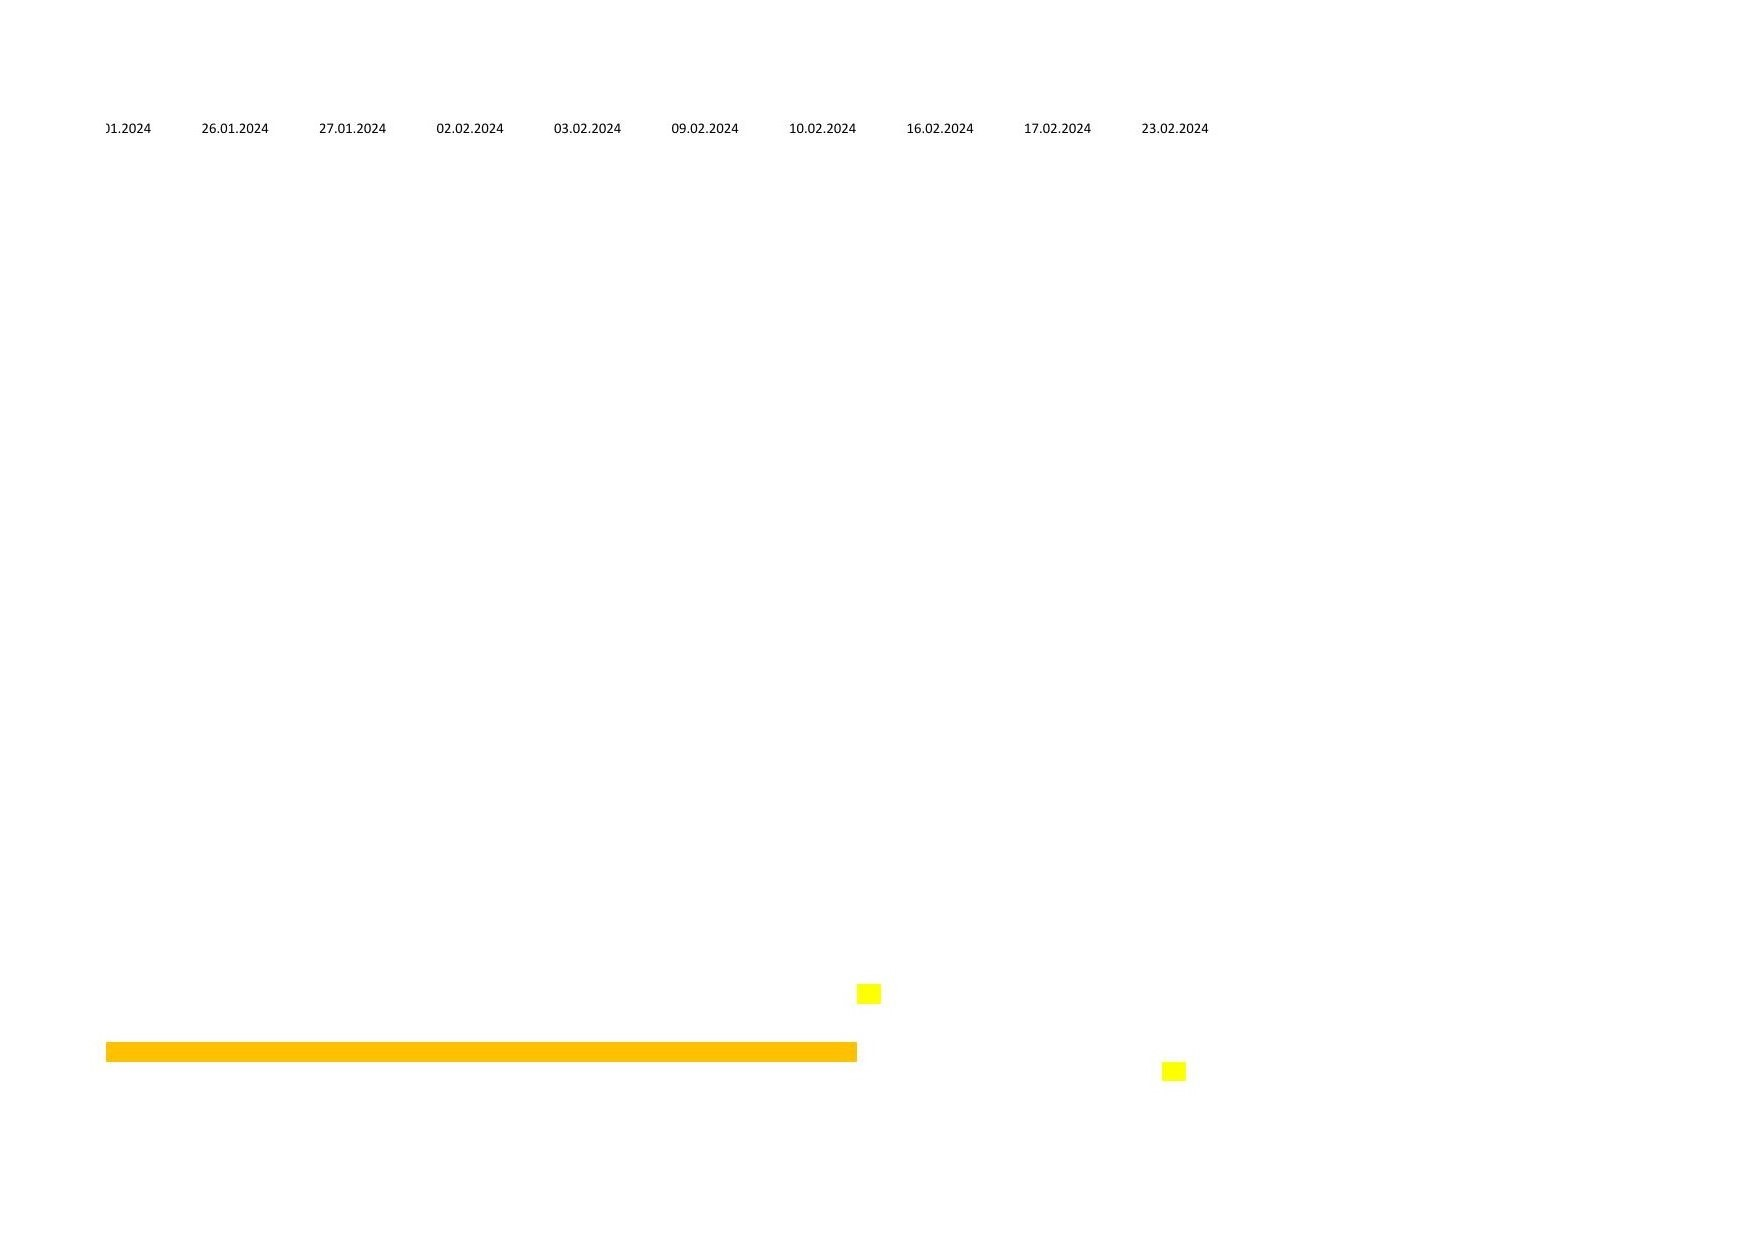
\includegraphics[width=\linewidth, height=\textheight, keepaspectratio]{gantt4_turned.jpg}
		\label{fig:gantt4}
	\end{figure}

\end{landscape}





%%Design
\chapter{Design}
\label{sec:Design}
\section{Konsole}
\label{sec:Konsole}
\subsection{Training}
\label{sec:Training}
\subsubsection{Input}
\label{sec:TraiInput}
\begin{lstlisting}[language=bash]
ki --training "[trainings.ubyte]"
\end{lstlisting}

\subsubsection{Output}
\label{sec:TraiOutput}
Nach jedem Datensatz wird angezeigt, wie viele der zum Training gegebenen Daten bereits abgearbeitet wurden. 

\subsection{Test}
\label{sec:Test}
\subsubsection{Input}
\label{sec:TestInput}
\begin{lstlisting}[language=bash]
ki --test "[test.ubyte]"
\end{lstlisting}

\subsubsection{Output}
\label{sec:TestOutput}
Nach jedem Datensatz wird angezeigt, wie viele der zum Testen gegebenen Daten bereits abgearbeitet wurden. Zudem wird angezeigt, wie viele der Datensatz richtig bzw. falsch erkannt wurden.



\subsection{Anwendung}
\label{sec:Anwendung}
\subsubsection{Input}
\label{sec:UseInput}
\begin{lstlisting}[language=bash]
ki "[image.jpg]"
\end{lstlisting}

\subsubsection{Output}
\label{sec:UseOutput}
Als Output werden alle Ziffern von 0 bis 9 mit den entsprechenden Prozentwerten zur�ckgegeben (Dies kommt daher, dass die KI die Wahrscheinlichkeit der �bereinstimmung f�r jede Ziffer berechnet.). Zudem wird auch angezeigt, welche Ziffer die h�chste �bereinstimmung hat. Da diese die erkannte Ziffer darstellt.

\section{Datenbank}
\label{sec:Datenbank}
Die Applikation ben�tigt keine Datenbank.

\section{Code}
\label{sec:Code}
\subsection{Klassendiagramm}
\label{sec:Klassendiagramm}
 Es gibt drei Klassen in CKi (Convolutional Layer, Pooling Layer, Dense Layers). Ein Convolutional Layer ist eine Art von Filter, welcher auf das Bild gelegt wird, um eine vereinfachte Erkennung zu erm�glichen. Die Pooling Layers sind verantwortlich das Bild zu verkleinern und so eine schnellere Verarbeitung zu erm�glichen. Die Dense Layers oder auch Fully Connected Layers sind das eigentlich das Gehirn der KI. Zus�tzlich gibt es die Main-Klasse, diese ist zust�ndig die oben genannten Klassen miteinander zu verbinden und so das Netzwerk aufzubauen. Zus�tzlich handhabt es die Nutzereingaben und die Auslese der Trainings-/Testdaten. 

\begin{figure}[H]
\centering
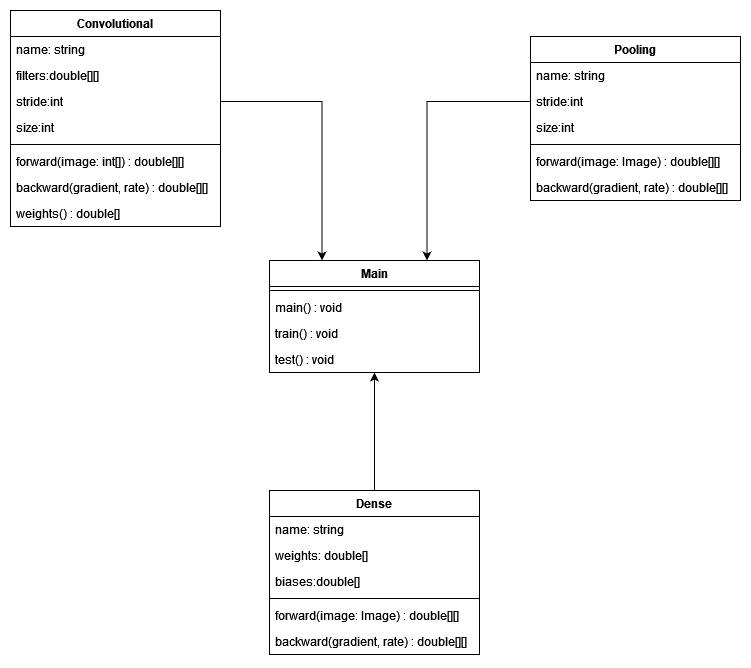
\includegraphics[height=0.5\paperheight]{Klassendiagramm.png}
\caption{Das Klassendiagramm, Grundaufbau der Applikation}
\label{fig:klassendiagramm}
\end{figure}

\subsection{Trainingsdaten}
\label{sec:Trainingsdaten}
Die Trainingsdaten sind das MNIST-Datenset mit den handschriftlichen Zahlen. (\url{http://yann.lecun.com/exdb/mnist/})

\subsection{Tests}
\label{sec:Tests}



%%Design
\chapter{Auftragsbezeichnung}
\label{sec:Auftrag}
\section{Identifikation}
\begin{xltabular}{\linewidth}{|l|l|}
	\hline
	Auftragsnummer & 
	\\\hline
	Auftragsbezeichnung & <Auftragsbezeichnung>
	\\\hline
\end{xltabular}
\label{tab:IdentifikationTable}

\section{Beschrieb des Ablaufs der Arbeit}
Für mein Projekt, das sich auf die Erforschung und Implementierung von Convolutional Neural Networks (CNN) und allgemeinen neuronalen Netzwerken konzentrierte, habe ich mich eigenständig auf eine umfassende Recherche eingelassen. Die Frist war die einzige Vorgabe, was mir die Freiheit liess, meine Interessen vollständig zu verfolgen. Grundlagenwissen zu CNNs und neuronalen Netzwerken sammelte ich durch sorgfältige Recherche auf renommierten Plattformen wie Medium, IBM, Geekflare, der Stanford University, und Database Camp. Bei der Lösung spezifischer Softwareprobleme erwiesen sich Stack Overflow, GitHub Copilot und ChatGPT, sowie die Dokumentationen der verwendeten Abhängigkeiten und Cppreference als unverzichtbare Ressourcen. Der Datensatz, der für das Training des Netzwerks verwendet wurde, stammt von Yann LeCun’s MNIST-Datenbank, einem Standardbenchmark in der Branche.
\\
Die Visualisierung des Projekts erfolgte durch die Erstellung von Ablaufdiagrammen, die sowohl den Prozess als auch die Struktur der Architektur eines neuronalen Netzwerks darstellen, sowie einem Klassendiagramm, das die objektorientierte Struktur der Implementierung verdeutlicht. Da keine Datenbank beteiligt war, wurde kein Entity-Relationship-Modell (ERM) benötigt.
\begin{figure}[H]
	\centering
		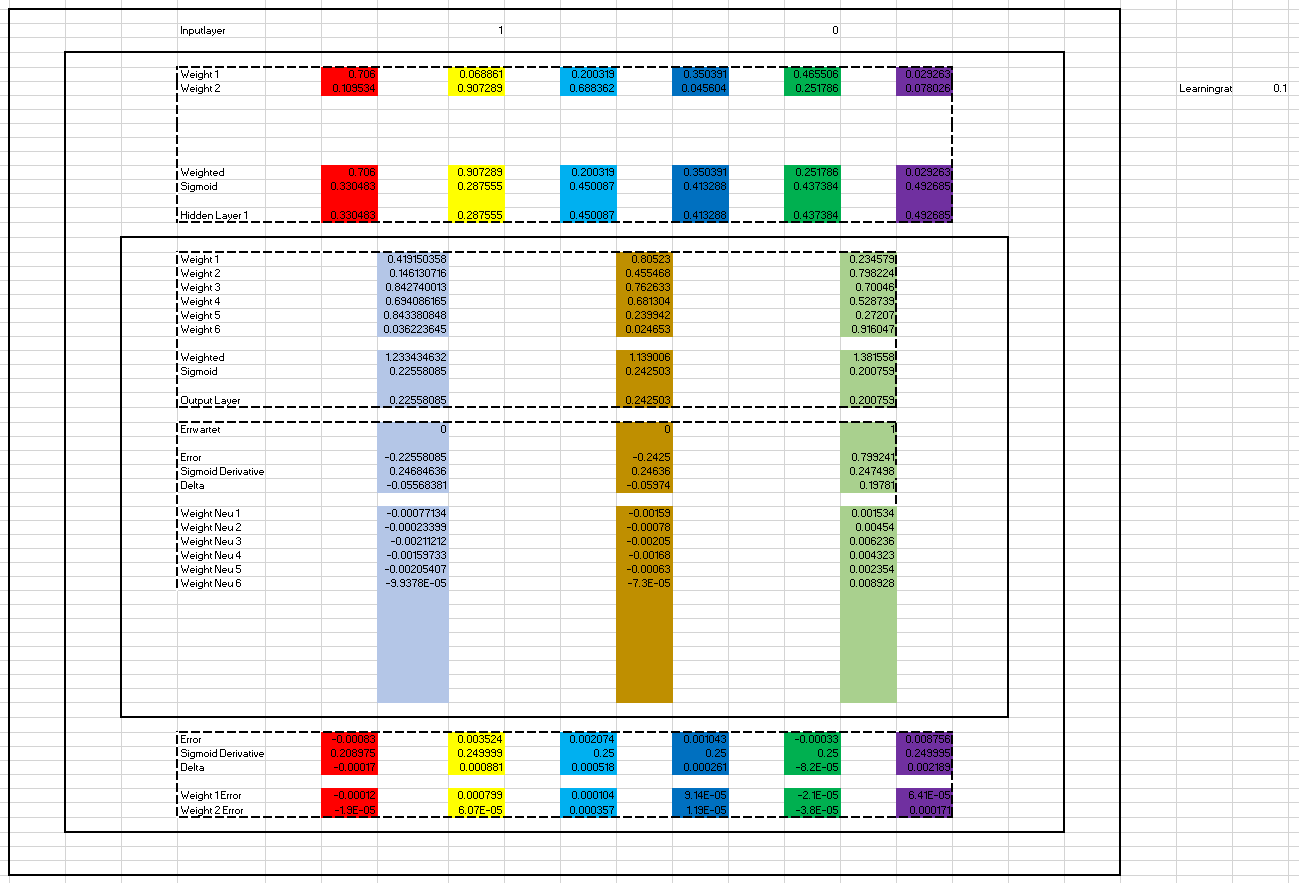
\includegraphics[width=\linewidth]{visualisierungKI.png}
		\caption{Meine Visualisierung eines neuronalen Netzwerkes in Excel.}
	\label{fig:visualisierungKI}
\end{figure}
\\
Die Entscheidung, das Projekt in C++ zu entwickeln, war nicht zufällig, sondern eine bewusste Wahl, die von mehreren Schlüsselfaktoren beeinflusst wurde. Zunächst ist C++ bekannt für seine aussergewöhnliche Leistungsfähigkeit und Effizienz\footnote{Zeigler, 1995; Hudak, 1994}, was es zur idealen Sprache für rechenintensive Anwendungen wie neuronale Netzwerke macht. Meine persönliche Vorliebe für C++ spielte ebenfalls eine Rolle. Überdies eröffnete die Wahl von C++ die Möglichkeit, in Zukunft die Verarbeitungsgeschwindigkeit durch die Einbindung von GPU-Berechnungen zu steigern. Dies wäre ein entscheidender Vorteil für die Skalierung und Effizienz des Projekts. Entwickelt wurde das Ganze unter Windows 11 und Manjaro Linux, einem Arsch-basierten Betriebssystem, mit CLion, einer IDE von JetBrains. Diese Entwicklungsumgebung wurde speziell wegen ihrer Benutzerfreundlichkeit und Cross-Plattform-Unterstützung ausgewählt, was einen nahtlosen Entwicklungsprozess auf verschiedenen Systemen ermöglichte. 
\\
Die Durchführung der Softwaretests erfolgte mittels des Google Test Frameworks, wodurch eine gründliche Prüfung jeder Klasse gewährleistet wurde. Dieser Ansatz trug entscheidend zur Stabilität und Funktionsfähigkeit des entwickelten Systems bei. Obwohl es keinen direkten Kunden für das Projekt gab, entschied ich mich dafür, den Quellcode auf Plattformen wie GitHub und GitLab zu teilen. Dieser Schritt diente nur der Demonstration meiner Arbeit und nicht dem Anstossen von Diskussionen, da dieses Projekt schon vielfach implementiert wurde. Es ist schliesslich das Einsteigerprojekt für Maschine Learning.

\section{Gemachte Erfahrungen}
\subsection{Im Bezug auf die ausgeführte Arbeit}
Im Rahmen des Projekts CKI zur Digitalisierung handschriftlicher Zahlen wurde eine umfassende Analyse der Herausforderungen und Erfahrungen durchgeführt. Die Komplexität der Problemstellung offenbarte sich in der tiefgreifenden Auseinandersetzung mit Maschine-Learning-Algorithmen und der fortgeschrittenen Programmierung in C++. Die Implementierung des Back-Propagation-Algorithmus stellte eine signifikante Hürde dar, deren Überwindung nicht nur technisches Verständnis, sondern auch eine methodische Herangehensweise erforderte. Technische Schwierigkeiten, wie die Integration externer C++-Bibliotheken und die Handhabung von Pointer-Exceptions, unterstrichen die Notwendigkeit einer präzisen Planung und Ausführung. Die Projektarbeit machte deutlich, dass die Erreichung einer hohen Präzision in der Zahlenidentifizierung eng mit der effizienten Nutzung der Ressourcen und der Minimierung von Rechenleistungsverbrauch verbunden ist. Trotz der Herausforderungen bot das Projekt wertvolle Einblicke in das Machine Learning.
\begin{figure}[htbp]
	\centering
		
\includegraphics{runtimeerror.png}
	\label{fig:runtimeerror}
\end{figure}

\subsection{Im Bezug auf das eigene Verhalten}
Diese Arbeit war zugleich motivierend und herausfordernd. Die Programmierung in C++ und die erfolgreiche Umsetzung des Projekts, insbesondere die Realisierung des neuronalen Netzwerks, haben mich sehr motiviert. Es war faszinierend, die direkten Auswirkungen meiner Arbeit zu sehen, vorwiegend bei der Erkennung handschriftlicher Ziffern. Jedoch hatten langwierige Probleme, wie die Implementierung der Back-Propagation, einen zermürbenden Effekt auf mich. Diese komplexen Herausforderungen erforderten viel Geduld und Ausdauer, und es gab Momente, in denen ich mich stark demotiviert fühlte.
\\
Des Weiteren empfand ich das Dokumentieren als eine beschwerliche Angelegenheit. Obwohl ich weiss, wie wichtig eine gute Dokumentation für die Nachvollziehbarkeit und Wartbarkeit eines Projekts ist, fiel es mir schwer, mich dazu zu motivieren. Meine Stärken liegen eindeutig in der praktischen Umsetzung – in der Realisation. Der Entwicklungsprozess, vornehmlich die Programmierung, hat mir viel Freude bereitet und ich habe gerne neue Funktionen implementiert und das Netzwerk optimiert.
\\
Allerdings habe ich gemerkt, dass ich dazu neige, schwierigere und anstrengender zu implementierende Teile, wie die Gestaltung der Benutzeroberfläche und die Implementierung der Back-Propagation, aufzuschieben. Diese Tendenz zum Aufschieben komplexerer Aufgaben hat mich in meiner Effizienz eingeschränkt und führte dazu, dass ich primär nur die unbedingt notwendigen Funktionen (Must-haves) implementierte. In Retrospektive sehe ich, dass ich zu viel prokrastiniert habe, was meine Zufriedenheit mit der eigenen Leistung mindert.
\\
Insgesamt bin ich mit dem, was ich erreicht habe, zufrieden, insbesondere mit der Realisierung des neuronalen Netzwerks, jedoch hätte ich mit mehr Durchhaltevermögen und einem besseren (Zeit-)Management mehr erreichen können.


\section{Lernergebnisse}
\subsection{Fach- und Methodenkompetenz}
<Was konnte ich fachlich dazu lernen?>
<In welchen Gebieten kenne ich mich nun aus, finde ich mich zurecht?>
\subsection{Selbst- und Sozialkompetenz}
<Was habe ich bezüglich meinem Verhalten mir gegenüber gelernt?>
<Was habe ich bezüglich meinem Verhalten anderen gegenüber gelernt?>
<Habe ich Kollegen, Lehrer, Fachpersonen genervt, gelangweilt, übermässig gestört, bloss gestellt, zu stark oder zu wenig respektiert, unterstützt, Anerkennung gegeben, belastet, entlastet und habe ich daraus etwas gelernt?>

\section{Schlussfolgerungen}
\subsection{Ziele, die ich errecihen will}
<Was möchte ich mehr wissen, können oder tun?>
<Was sollte weniger passieren?>
\subsection{Termin der Zielüberprüfung}
<Bis wann werde ich die Ziele erreicht haben?>

\section{Bemerkungen}
< Was wäre wichtig, ist aber noch nicht angesprochen worden?>

\section{Weiterführende Aktionen}
<Was gibt es noch zu tun?>
<Was konnte wieso nicht gemacht werden?>



%% weitere Verzeichnisse 
%%\addtocontents{toc}{\protect\vspace*{\baselineskip}}

%% Literaturverzeichnis
%% ==> Eine Datei 'literatur.bib' wird hierfür benötigt.
%% ==> Sie müssen hierfür BibTeX verwenden (Projekt | Eigenschaften... | BibTeX)
\clearpage
\addcontentsline{toc}{chapter}{Literaturverzeichnis}
%%\addbibresource{literatur.bib}
\nocite{*} %Auch nicht-zitierte BibTeX-Einträge werden angezeigt.
\bibliographystyle{plain} %Art der Ausgabe: plain / apalike / amsalpha / ...
\bibliography{literatur} %Eine Datei 'literatur.bib' wird hierfür benötigt.

%% Abbildungsverzeichnis
\clearpage
\addcontentsline{toc}{chapter}{Abbildungsverzeichnis}
\listoffigures

%% Tabellenverzeichnis
%\clearpage
%\addcontentsline{toc}{chapter}{Tabellenverzeichnis}
%\listoftables


%% Anhänge
%%\appendix

\end{document}

